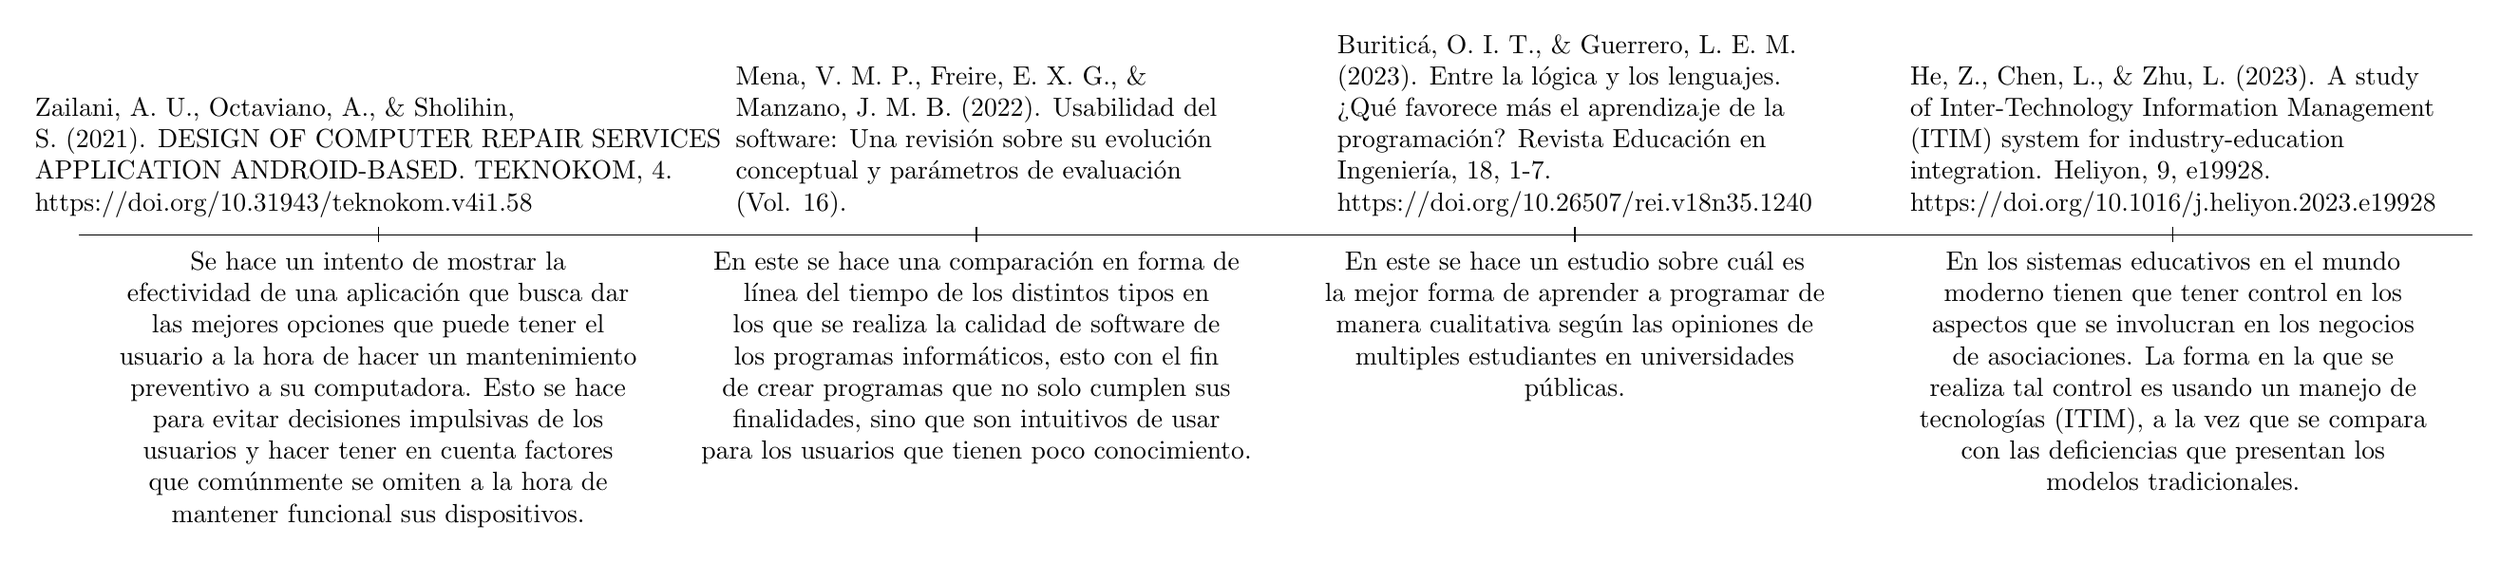
\begin{tikzpicture}
% draw a horizontal line
\draw (0,0) -- (32,0);
% draw vertical lines
\foreach \x in {4,12,20,28}
\draw (\x cm,3pt) -- (\x cm,-3pt);

% draw nodes to add events
\draw (0,0) -- (32,0);
% draw vertical lines
\foreach \x in {4,12,20,28}
\draw (\x cm,3pt) -- (\x cm,-3pt);

% draw nodes to add events
\draw (4,0) node[below=3pt, align=center] {
  Se hace un intento de mostrar la \\
  efectividad de una aplicación que busca dar \\
  las mejores opciones que puede tener el \\
  usuario a la hora de hacer un mantenimiento \\
  preventivo a su computadora. Esto se hace \\
  para evitar decisiones impulsivas de los \\
  usuarios y hacer tener en cuenta factores \\
  que comúnmente se omiten a la hora de \\
  mantener funcional sus dispositivos.
} 
node[above=3pt, align=left] {
  Zailani, A. U., Octaviano, A., \& Sholihin,\\
  S. (2021). DESIGN OF COMPUTER REPAIR SERVICES\\
  APPLICATION ANDROID-BASED. TEKNOKOM, 4.\\
  https://doi.org/10.31943/teknokom.v4i1.58
};
\draw (12,0) node[below=3pt, align=center] {
  En este se hace una comparación en forma de \\
  línea del tiempo de los distintos tipos en \\
  los que se realiza la calidad de software de \\
  los programas informáticos, esto con el fin \\
  de crear programas que no solo cumplen sus \\
  finalidades, sino que son intuitivos de usar \\
  para los usuarios que tienen poco conocimiento.
} node[above=3pt, align=left] {
  Mena, V. M. P., Freire, E. X. G., \&\\
  Manzano, J. M. B. (2022). Usabilidad del\\
  software: Una revisión sobre su evolución\\
  conceptual y parámetros de evaluación\\
  (Vol. 16).
};
\draw (20,0) node[below=3pt, align=center] {
  En este se hace un estudio sobre cuál es \\
  la mejor forma de aprender a programar de \\
  manera cualitativa según las opiniones de \\
  multiples estudiantes en universidades \\
  públicas.
} node[above=3pt, align=left] {
  Buriticá, O. I. T., \& Guerrero, L. E. M.\\
  (2023). Entre la lógica y los lenguajes.\\
  ¿Qué favorece más el aprendizaje de la\\
  programación? Revista Educación en\\
  Ingeniería, 18, 1-7.\\
  https://doi.org/10.26507/rei.v18n35.1240
};
\draw (28,0) node[below=3pt, align=center] {
  En los sistemas educativos en el mundo \\
  moderno tienen que tener control en los \\
  aspectos que se involucran en los negocios \\
  de asociaciones. La forma en la que se \\
  realiza tal control es usando un manejo de \\
  tecnologías (ITIM), a la vez que se compara \\
  con las deficiencias que presentan los \\
  modelos tradicionales.
} node[above=3pt, align=left] {
  He, Z., Chen, L., \& Zhu, L. (2023). A study\\
  of Inter-Technology Information Management\\
  (ITIM) system for industry-education\\
  integration. Heliyon, 9, e19928.\\
  https://doi.org/10.1016/j.heliyon.2023.e19928
};
\end{tikzpicture}
